\chapter{Theory}
	Going through the theory in the book \textit{Sensation and perception}, to categorize the different depth cues a tree was made, and to give structure to my essay, I remade a copy of it as seen \autoref{fig:depthCues}, and will utilize this for presenting my findings and answering the topic questions.
	\begin{figure}[H]
		\centering
		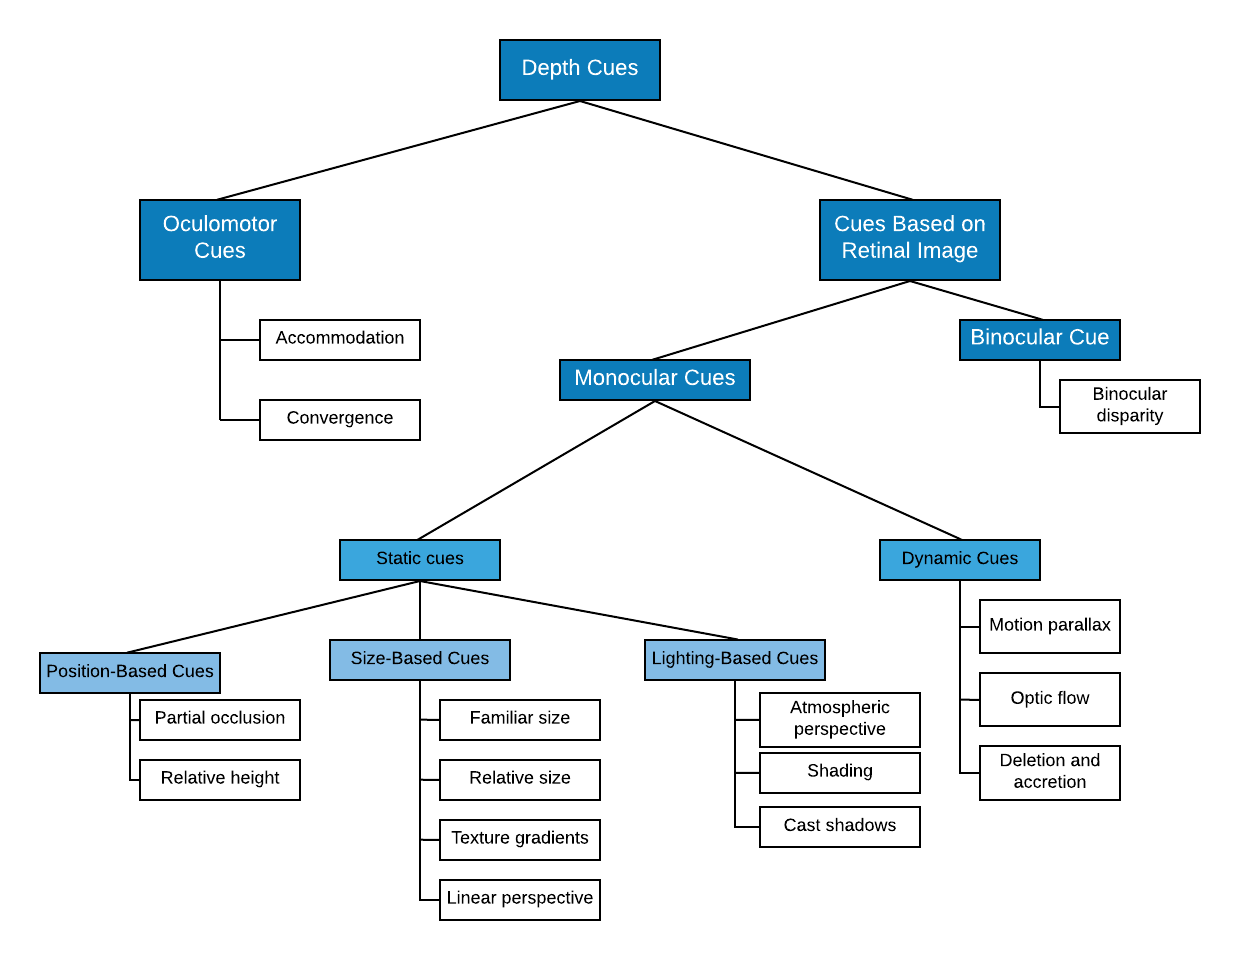
\includegraphics[width=1\linewidth]{figure/depthcues}
		\caption{All the depth cues from the book, Sensation and Perception\citep{sensationPerception}, the figure was made as a copy from the figure on page 195.}
		\label{fig:depthCues}
	\end{figure}
	\section{Oculomotor cues}
		Information from muscles in the eye and such
	\section{Retinal image cues}
		Retinal image information
		\subsection{Static cues}
			No movement
		\subsection{Dynamic cues}
			Movement
	\section{Stereopsis}
		
		\subsection{binocular disparity}
		Difference between the eyes and shit
		
		\subsection*{stereograms}
		
		\subsection*{Autostereograms}